\documentclass[../main.tex]{subfiles}

\begin{document}

\textbf{Hatcher 0.10.} \par
Suppose $X$ is contractible, $\{*\}$ is the one point space, $\exists \varphi:X\rightarrow \{*\}, \psi:\{*\}\rightarrow X$ such that $\psi\circ\varphi \simeq \mathrm{id}_{X}$, thus for any map $f:X\rightarrow Y$ and arbitrary space $Y$ we have $ f= f\circ\mathrm{id}_{X} \simeq f\circ\psi\varphi $ where \(\psi\varphi\) is constant map, hence $f$ is nullhomotopic. Conversely, suppose for any map $f:X\rightarrow Y$ and arbitrary space $Y$, $f$ is nullhomotopic. Take $Y$ to be $X$, and $f$ to be $\mathrm{id}_{X}$, then $\mathrm{id}_{X}\simeq c_{x_{0}}$ where $x_{0}\in X$ and $c_{x_{0}}$ is the constant map, define $\varphi:X\rightarrow \{*\}$ by $\varphi(x)=*$ for any $x\in X$, and define $\psi:\{*\}\rightarrow X$ by $\psi(*)=x_{0}$, then $\psi\circ\varphi=c_{x_{0}}\simeq\mathrm{id}_{X}$ and $\psi\circ\varphi=\mathrm{id}_{\{*\}}$, hence $X$ is contractible.
Similarly, suppose $X$ is contractible, $\{*\}$ is the one point space, $\exists \varphi:Y\rightarrow \{*\}, \psi:\{*\}\rightarrow Y$ such that $\psi\circ\varphi \simeq \mathrm{id}_{Y}$, thus for any map $f:Y\rightarrow X$ and arbitrary space $Y$ we have $ f=f\circ\mathrm{id}_{Y}\simeq f\circ\psi\varphi $ where \(\psi\varphi\) is constant map, hence $f$ is nullhomotopic. Conversely, suppose for any map $f:Y\rightarrow X$ and arbitrary space $Y$, $f$ is nullhomotopic. Take $Y$ to be $X$, and $f$ to be $\mathrm{id}_{X}$, then $\mathrm{id}_{X}\simeq c_{x_{0}}$ where $x_{0}\in X$ and $c_{x_{0}}$ is the constant map, define $\varphi:X\rightarrow \{*\}$ by $\varphi(x)=*$ for any $x\in X$, and define $\psi:\{*\}\rightarrow X$ by $\psi(*)=x_{0}$, then $\psi\circ\varphi=c_{x_{0}}\simeq\mathrm{id}_{X}$ and $\psi\circ\varphi=\mathrm{id}_{\{*\}}$, hence $X$ is contractible.

\textbf{Hatcher 0.14.} \par
Since $f\geq 1$, $1\geq 2-f= v-e\Rightarrow e\geq v-1 $, hence we can construct as follows, where $x_{1},\cdots,x_{v}$ are 0-cells, and $l_{1},\cdots,l_{e}$ are 1-cells, which divide $\mathbb{S}^{2}$ into $f$ 2-cells, and this give $\mathbb{S}^{2}$ a CW complex structure as we wanted.
\begin{center}
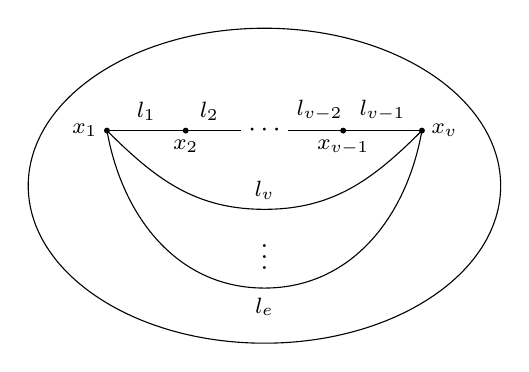
\begin{tikzpicture}
\draw (0,-0.7) ellipse (3 and 2);
\node [below,left] at (-2,0) {\footnotesize $x_{1}$};
\draw[fill] (-2,0) circle [radius=0.03];
\node [below] at (-1,0) {\footnotesize $x_{2}$};
\draw[fill] (-1,0) circle [radius=0.03];
\node [below] at (1,0) {\footnotesize $x_{v-1}$};
\draw[fill] (1,0) circle [radius=0.03];
\node [below,right] at (2,0) {\footnotesize $x_{v}$};
\draw[fill] (2,0) circle [radius=0.03];
\draw(-2,0)--(-1,0);
\node [above] at (-1.5,0) {\footnotesize $l_{1}$};
\draw(1,0)--(2,0);
\node [above] at (1.5,0) {\footnotesize $l_{v-1}$};
\draw(-1,0)--(-0.3,0);
\node [above] at (-0.7,0) {\footnotesize $l_{2}$};
\draw(0.3,0)--(1,0);
\node [above] at (0.7,0) {\footnotesize $l_{v-2}$};
\node at (0,0) {$\cdots$};
\node at (0,-1.5) {$\vdots$};
\draw (-2,0) to [out=-45,in=-180] (0,-1) node [above] {\footnotesize $l_{v}$} to [out=0,in=-135] (2,0);
\draw (-2,0) to [out=-80,in=-180] (0,-2) node [below] {\footnotesize $l_{e}$} to [out=0,in=-100] (2,0);
\end{tikzpicture}
\end{center}

\textbf{Hatcher 1.1.1} \par
Since $g_{0}\simeq g_{1}$, there exists continuous map $H:I\times I\rightarrow X$, such that $H(s,0)=g_{0}(s), H(s,1)=g_{1}(s)$, then $\overline{H}(s,t):=H(1-s,t)$ is so a continuous map from $I\times I$ to $X$ with $\overline{H}(s,0)=\overline{g_{0}}(s), \overline{H}(s,1)=\overline{g_{1}}(s)$, thus $\overline{g_{0}}\simeq\overline{g_{1}}$, hence $f_{0}=f_{0}\cdot g_{0}\cdot \overline{g_{0}}\simeq f_{1}\cdot g_{1}\cdot \overline{g_{1}}=f_{1}$

\textbf{1.} \par
\begin{center}
\begin{tikzcd}
\mathbb{S}^{n-1} \arrow[r,hook,"i"]
& \mathbb{R}^{n}\setminus\{0\} \arrow[r,"\pi"] 
& \mathbb{S}^{n-1} 
\end{tikzcd}
\end{center}
Where $i$ is inclusion map and $\pi$ is given by $\pi(x)=\dfrac{x}{|x|}$, then $\pi\circ i=\mathrm{id}_{\mathbb{S}^{n-1} }$, and $i\circ\pi\simeq\mathrm{id}_{\mathbb{R}^{n}\setminus\{0\} }$ by homotopy $H:\mathbb{R}^{n}\setminus\{0\}\times I \rightarrow \mathbb{R}^{n}\setminus\{0\}, (x,t)\mapsto tx+(1-t)\dfrac{x}{|x|}$, which demonstrate $\mathbb{S}^{n-1} \simeq\mathbb{R}^{n}\setminus\{0\} $ \par
\textbf{2.} \par
$H:\mathbb{S}^{n}\setminus N\times I\rightarrow\mathbb{S}^{n}\setminus N$, given by \[ H(x,t)=\left( \dfrac{x}{|x|}\sqrt{1-\left(tx_{n+1}-(1-t)\right)^{2}}, tx_{n+1}-(1-t) \right) \] Where $N$ is north pole.
$H$ is a homotopy between $\mathrm{id}_{\mathbb{S}^{n}\setminus N}$ and $c_{N}$, where $c_{N}$ is the constant map that maps $\mathbb{S}^{n}\setminus N$ to $N$, thus $\mathrm{id}_{\mathbb{S}^{n}\setminus N}\simeq c_{N}$. Since $\phi$ is continuous but not surjective, we can assume $N\notin \phi(\mathbb{S}^{n})$, then $\phi\simeq\mathrm{id}_{\mathbb{S}^{n}\setminus N}\circ\phi\simeq c_{N}\circ\phi$, hence $\phi$ is nullhomotopic. \par
\textbf{3.} \par
If $n$ is odd, then $n+1$ is even, then we could define $H:\mathbb{S}^{n}\times I\rightarrow \mathbb{S}^{n}$ by rotating the first two coordinates while fix the rest, written explictly \[H(x_{1},x_{2},\cdots,x_{n+1})=\left(x_{1}\cos{\pi t}-x_{2}\sin{\pi t}, x_{1}\sin{\pi t}+x_{2}\cos{\pi t}, \cdots, x_{n+1}\right)\] The remaining coordinates are of even number, thus we could could repeat this process $\dfrac{n+1}{2}$ times, and compose all these homotopy, thus shows that $a\simeq\mathrm{id}_{\mathbb{S}^{n}}$ \par
\textbf{4.} \par
Reflexivity: Suppose $f:X\rightarrow Y$, then \(f\overset{H}{\simeq}f,\mathrm{rel}\,Z\), where $H(x,t)=f(x)$ \par
Symmetry: Suppose $f,g:X\rightarrow Y$, and \(f\overset{H}{\simeq}g,\mathrm{rel}\,Z\), then \(g\overset{H'}{\simeq}f,\mathrm{rel}\,Z\) where $H'(x,t)=H(x,1-t)$ \par
Transitivity: Suppose $f,g,h:X\rightarrow Y$, and \(f\overset{F}{\simeq}g,\mathrm{rel}\,Z\),  \(g\overset{G}{\simeq}h,\mathrm{rel}\,Z\), then  \(f\overset{H}{\simeq}h,\mathrm{rel}\,Z\), where\[
H(x,t)=
\left\{\begin{matrix}
F\left(x,2t\right), t\in\left[0,\frac{1}{2}\right]\\ 
G\left(x,2t-1\right), t\in\left[\frac{1}{2},1\right]
\end{matrix}\right.
\]
Therefore, homotopy relative a given subspace $Z\subset X$ is an equivalence relation on the set of maps from $X$ to $Y$

\end{document}